% Options for packages loaded elsewhere
\PassOptionsToPackage{unicode}{hyperref}
\PassOptionsToPackage{hyphens}{url}
\PassOptionsToPackage{dvipsnames,svgnames,x11names}{xcolor}
\documentclass[
  10pt,
  fontset=fandol]{ctexart}
\usepackage{xcolor}
\usepackage[margin=16mm]{geometry}
\usepackage{amsmath,amssymb}
\setcounter{secnumdepth}{-\maxdimen} % remove section numbering
\usepackage{iftex}
\ifPDFTeX
  \usepackage[T1]{fontenc}
  \usepackage[utf8]{inputenc}
  \usepackage{textcomp} % provide euro and other symbols
\else % if luatex or xetex
  \usepackage{unicode-math} % this also loads fontspec
  \defaultfontfeatures{Scale=MatchLowercase}
  \defaultfontfeatures[\rmfamily]{Ligatures=TeX,Scale=1}
\fi
\usepackage{lmodern}
\ifPDFTeX\else
  % xetex/luatex font selection
\fi
% Use upquote if available, for straight quotes in verbatim environments
\IfFileExists{upquote.sty}{\usepackage{upquote}}{}
\IfFileExists{microtype.sty}{% use microtype if available
  \usepackage[]{microtype}
  \UseMicrotypeSet[protrusion]{basicmath} % disable protrusion for tt fonts
}{}
\makeatletter
\@ifundefined{KOMAClassName}{% if non-KOMA class
  \IfFileExists{parskip.sty}{%
    \usepackage{parskip}
  }{% else
    \setlength{\parindent}{0pt}
    \setlength{\parskip}{6pt plus 2pt minus 1pt}}
}{% if KOMA class
  \KOMAoptions{parskip=half}}
\makeatother
\usepackage{longtable,booktabs,array}
\newcounter{none} % for unnumbered tables
\usepackage{calc} % for calculating minipage widths
% Correct order of tables after \paragraph or \subparagraph
\usepackage{etoolbox}
\makeatletter
\patchcmd\longtable{\par}{\if@noskipsec\mbox{}\fi\par}{}{}
\makeatother
% Allow footnotes in longtable head/foot
\IfFileExists{footnotehyper.sty}{\usepackage{footnotehyper}}{\usepackage{footnote}}
\makesavenoteenv{longtable}
\usepackage{graphicx}
\makeatletter
\newsavebox\pandoc@box
\newcommand*\pandocbounded[1]{% scales image to fit in text height/width
  \sbox\pandoc@box{#1}%
  \Gscale@div\@tempa{\textheight}{\dimexpr\ht\pandoc@box+\dp\pandoc@box\relax}%
  \Gscale@div\@tempb{\linewidth}{\wd\pandoc@box}%
  \ifdim\@tempb\p@<\@tempa\p@\let\@tempa\@tempb\fi% select the smaller of both
  \ifdim\@tempa\p@<\p@\scalebox{\@tempa}{\usebox\pandoc@box}%
  \else\usebox{\pandoc@box}%
  \fi%
}
% Set default figure placement to htbp
\def\fps@figure{htbp}
\makeatother
\setlength{\emergencystretch}{3em} % prevent overfull lines
\providecommand{\tightlist}{%
  \setlength{\itemsep}{0pt}\setlength{\parskip}{0pt}}
\usepackage{amsmath,amssymb,mathtools,needspace}
\xeCJKDeclareCharClass{CJK}{"2032,"0400->"04FF,"2160->"216B,"2460->"2473,"25A0,"25C7,"25CB,"25CF}
\IfFontExistsTF{Arial Unicode MS}{\xeCJKsetup{AutoFallBack=true}\setCJKfallbackfamilyfont{\CJKrmdefault}{Arial Unicode MS}}{}
\setcounter{secnumdepth}{0}
\setlength{\emergencystretch}{2em}
\allowdisplaybreaks
\usepackage{bookmark}
\IfFileExists{xurl.sty}{\usepackage{xurl}}{} % add URL line breaks if available
\urlstyle{same}
\hypersetup{
  pdftitle={Euler 格式},
  colorlinks=true,
  linkcolor={Maroon},
  filecolor={Maroon},
  citecolor={Blue},
  urlcolor={Blue},
  pdfcreator={LaTeX via pandoc}}

\title{Euler 格式}
\author{}
\date{}

\begin{document}
\maketitle

\subsubsection{5.2.1 Euler 格式}\label{euler-ux683cux5f0f}

我们知道，在 \(Oxy\) 平面上，微分方程 (5.1.1) 的解 \(y=y(x)\) 称为它的\textbf{积分曲线}。积分曲线上一点 \((x,y)\) 的切线斜率等于函数 \(f(x,y)\) 的值。如果按函数 \(f(x,y)\) 在 \(Oxy\) 平面上建立一个方向场，那么，积分曲线上每一点的切线方向均与方向场在该点的方向一致。

基于上述几何解释，我们从初始点 \(P_0(x_0,y_0)\) 出发，先依方向场在该点的方向推

\href{../../source-images/pdf-120.jpeg}{原页}

进到 \(x=x_1\) 上一点 \(P_1\)，然后再从 \(P_1\) 依方向场的方向推进到 \(x=x_2\) 上一点 \(P_2\)，循此前进作出一条折线 \(P_0P_1P_2\cdots\)（见图 5.1）。

一般地，设已作出该折线的极点 \(P_n\)，过 \(P_n(x_n,y_n)\) 依方向场的方向再推进到 \(P_{n+1}(x_{n+1},y_{n+1})\)，显然两个极点 \(P_n,P_{n+1}\) 的坐标有下列关系：

\[
\frac{y_{n+1}-y_n}{x_{n+1}-x_n}=f(x_n,y_n),
\]

即

\[
y_{n+1}=y_n+hf(x_n,y_n).\tag{5.2.1}
\]

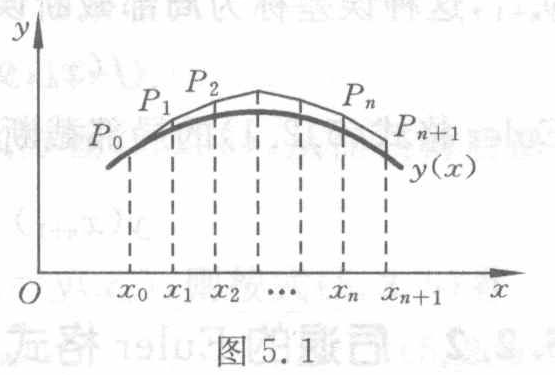
\includegraphics[width=0.85\linewidth,height=\textheight,keepaspectratio,alt={图 5.1 原图}]{../assets/ch05a/fig-5.1.png}

图 5.1（原图）：Euler 折线 \(P_0P_1P_2\cdots P_nP_{n+1}\) 与积分曲线 \(y(x)\)。原图符号标签：\(O,\allowbreak x,\allowbreak y,\allowbreak x_0,\allowbreak x_1,\allowbreak x_2,\allowbreak \cdots,\allowbreak x_n,\allowbreak x_{n+1},\allowbreak P_0,\allowbreak P_1,\allowbreak P_2,\allowbreak P_n,\allowbreak P_{n+1},\allowbreak y(x)\)。

这就是著名的 \textbf{Euler 格式}。若初值 \(y_0\) 已知，则依格式 (5.2.1) 可逐步算出

\[
y_1=y_0+hf(x_0,y_0),\qquad y_2=y_1+hf(x_1,y_1),\qquad\cdots.
\]

\textbf{例 5.1} 求解初值问题

\[
\begin{cases}
y'=y-2x/y\quad(0<x<1),\\
y(0)=1.
\end{cases}\tag{5.2.2}
\]

\textbf{解} 为便于比较，本章将用多种数值方法求解上述初值问题。这里先用 Euler 方法，Euler 格式的具体形式为

\[
y_{n+1}=y_n+h\left(y_n-\frac{2x_n}{y_n}\right).
\]

取步长 \(h=0.1\)，计算结果如表 5.1 所示。

\textbf{表 5.1}

{\def\LTcaptype{none} % do not increment counter
\begin{longtable}[]{@{}llllll@{}}
\toprule\noalign{}
\(x_n\) & \(y_n\) & \(y(x_n)\) & \(x_n\) & \(y_n\) & \(y(x_n)\) \\
\midrule\noalign{}
\endhead
\bottomrule\noalign{}
\endlastfoot
0.1 & 1.1000 & 1.0954 & 0.6 & 1.5090 & 1.4832 \\
0.2 & 1.1918 & 1.1832 & 0.7 & 1.5803 & 1.5492 \\
0.3 & 1.2774 & 1.2649 & 0.8 & 1.6498 & 1.6125 \\
0.4 & 1.3582 & 1.3416 & 0.9 & 1.7178 & 1.6733 \\
0.5 & 1.4351 & 1.4142 & 1.0 & 1.7848 & 1.7321 \\
\end{longtable}
}

初值问题 (5.2.2) 有解 \(y=\sqrt{1+2x}\)，按这个解析式子算出的准确值 \(y(x_n)\) 同近似值 \(y_n\) 一起列在表 5.1 中，二者相比较可以看出，Euler 方法的精度很差。

还可以通过几何直观来考察 Euler 方法的精度。假设 \(y_n=y(x_n)\)，即顶点 \(P_n\) 落在积分曲线 \(y=y(x)\) 上，那么，按 Euler 方法作出的折线 \(P_nP_{n+1}\) 便是 \(y=y(x)\) 过点 \(P_n\) 的切线（见图 5.2）。从图形上看，这样定出的顶点 \(P_{n+1}\) 显著地偏离了原来的积分曲线，可见 Euler 方法是相当粗糙的。

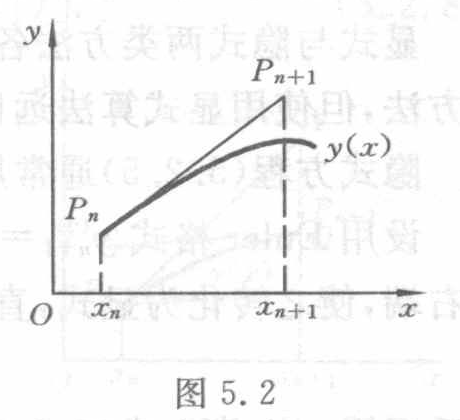
\includegraphics[width=0.85\linewidth,height=\textheight,keepaspectratio,alt={图 5.2 原图}]{../assets/ch05a/fig-5.2.png}

图 5.2（原图）：从积分曲线上 \(P_n\) 沿切线得到 \(P_{n+1}\)，与曲线 \(y(x)\) 在 \(x_{n+1}\) 的值有偏差。原图符号标签：\(O,\allowbreak x,\allowbreak y,\allowbreak x_n,\allowbreak x_{n+1},\allowbreak P_n,\allowbreak P_{n+1},\allowbreak y(x)\)。

人们常以 Taylor 展开为工具来分析计算公式的

\href{../../source-images/pdf-121.jpeg}{原页}

精度。为简化分析，假定 \(y_n\) 是准确的，即在 \(y_n=y(x_n)\) 的前提下估计误差 \(y(x_{n+1})-y_{n+1}\)，这种误差称为\textbf{局部截断误差}。注意到

\[
f(x_n,y_n)=f(x_n,y(x_n))=y'(x_n),
\]

Euler 格式 (5.2.1) 的局部截断误差显然为

\[
y(x_{n+1})-y_{n+1}=\frac{h^2}{2}y''(\xi)\approx\frac{h^2}{2}y''(x_n).\tag{5.2.3}
\]

\end{document}
